\section{Introduction}
Additive manufacturing (or 3D Printing) is an emerging technology, in which
materials are printed in layers having a 3D model as a reference. However this process is not always perfect and printing errors are to be expected. Manually reviewing every print job is a tedious labor work, hence automatization of this process is ??a nice improvement, cost/time saver??. \\
In this thesis a YOLOv5 \cite{yolov5_git} neural network solution is proposed and analyzed for this automatization procedure.
\par

\subsection{Printing process}
The 3D printer in ??our experiments uses binder jetting technology. With this technology, a layer is printed by laying a powder bed, then the printer applies drops of binding agent in regions of the bed to bond the powder particles together \cite{binder_jetting}. \\
In order to see the printing defects for each layer, our 3D printer had an internal camera that captured each layer. The captured images were then calibrated. In figure \ref{fig:layer_bitmask} a printed layer and the respective reference layer model can be seen. The aforementioned layer model is actually just a binary bitmask with each 1-valued pixel marking a one square millimeter region that must be printed.\\
In our case the printing errors are scratches on the printed surfaces like in figure \ref{fig:layer_00325_marked_cropped}. This scratches are from a visual perspective some dark vertical lines, that might extend over the printed region, however only the segments on the printed region are considered scratches.


\begin{figure}[ht]
  \centering

  \begin{subfigure}{\textwidth}
    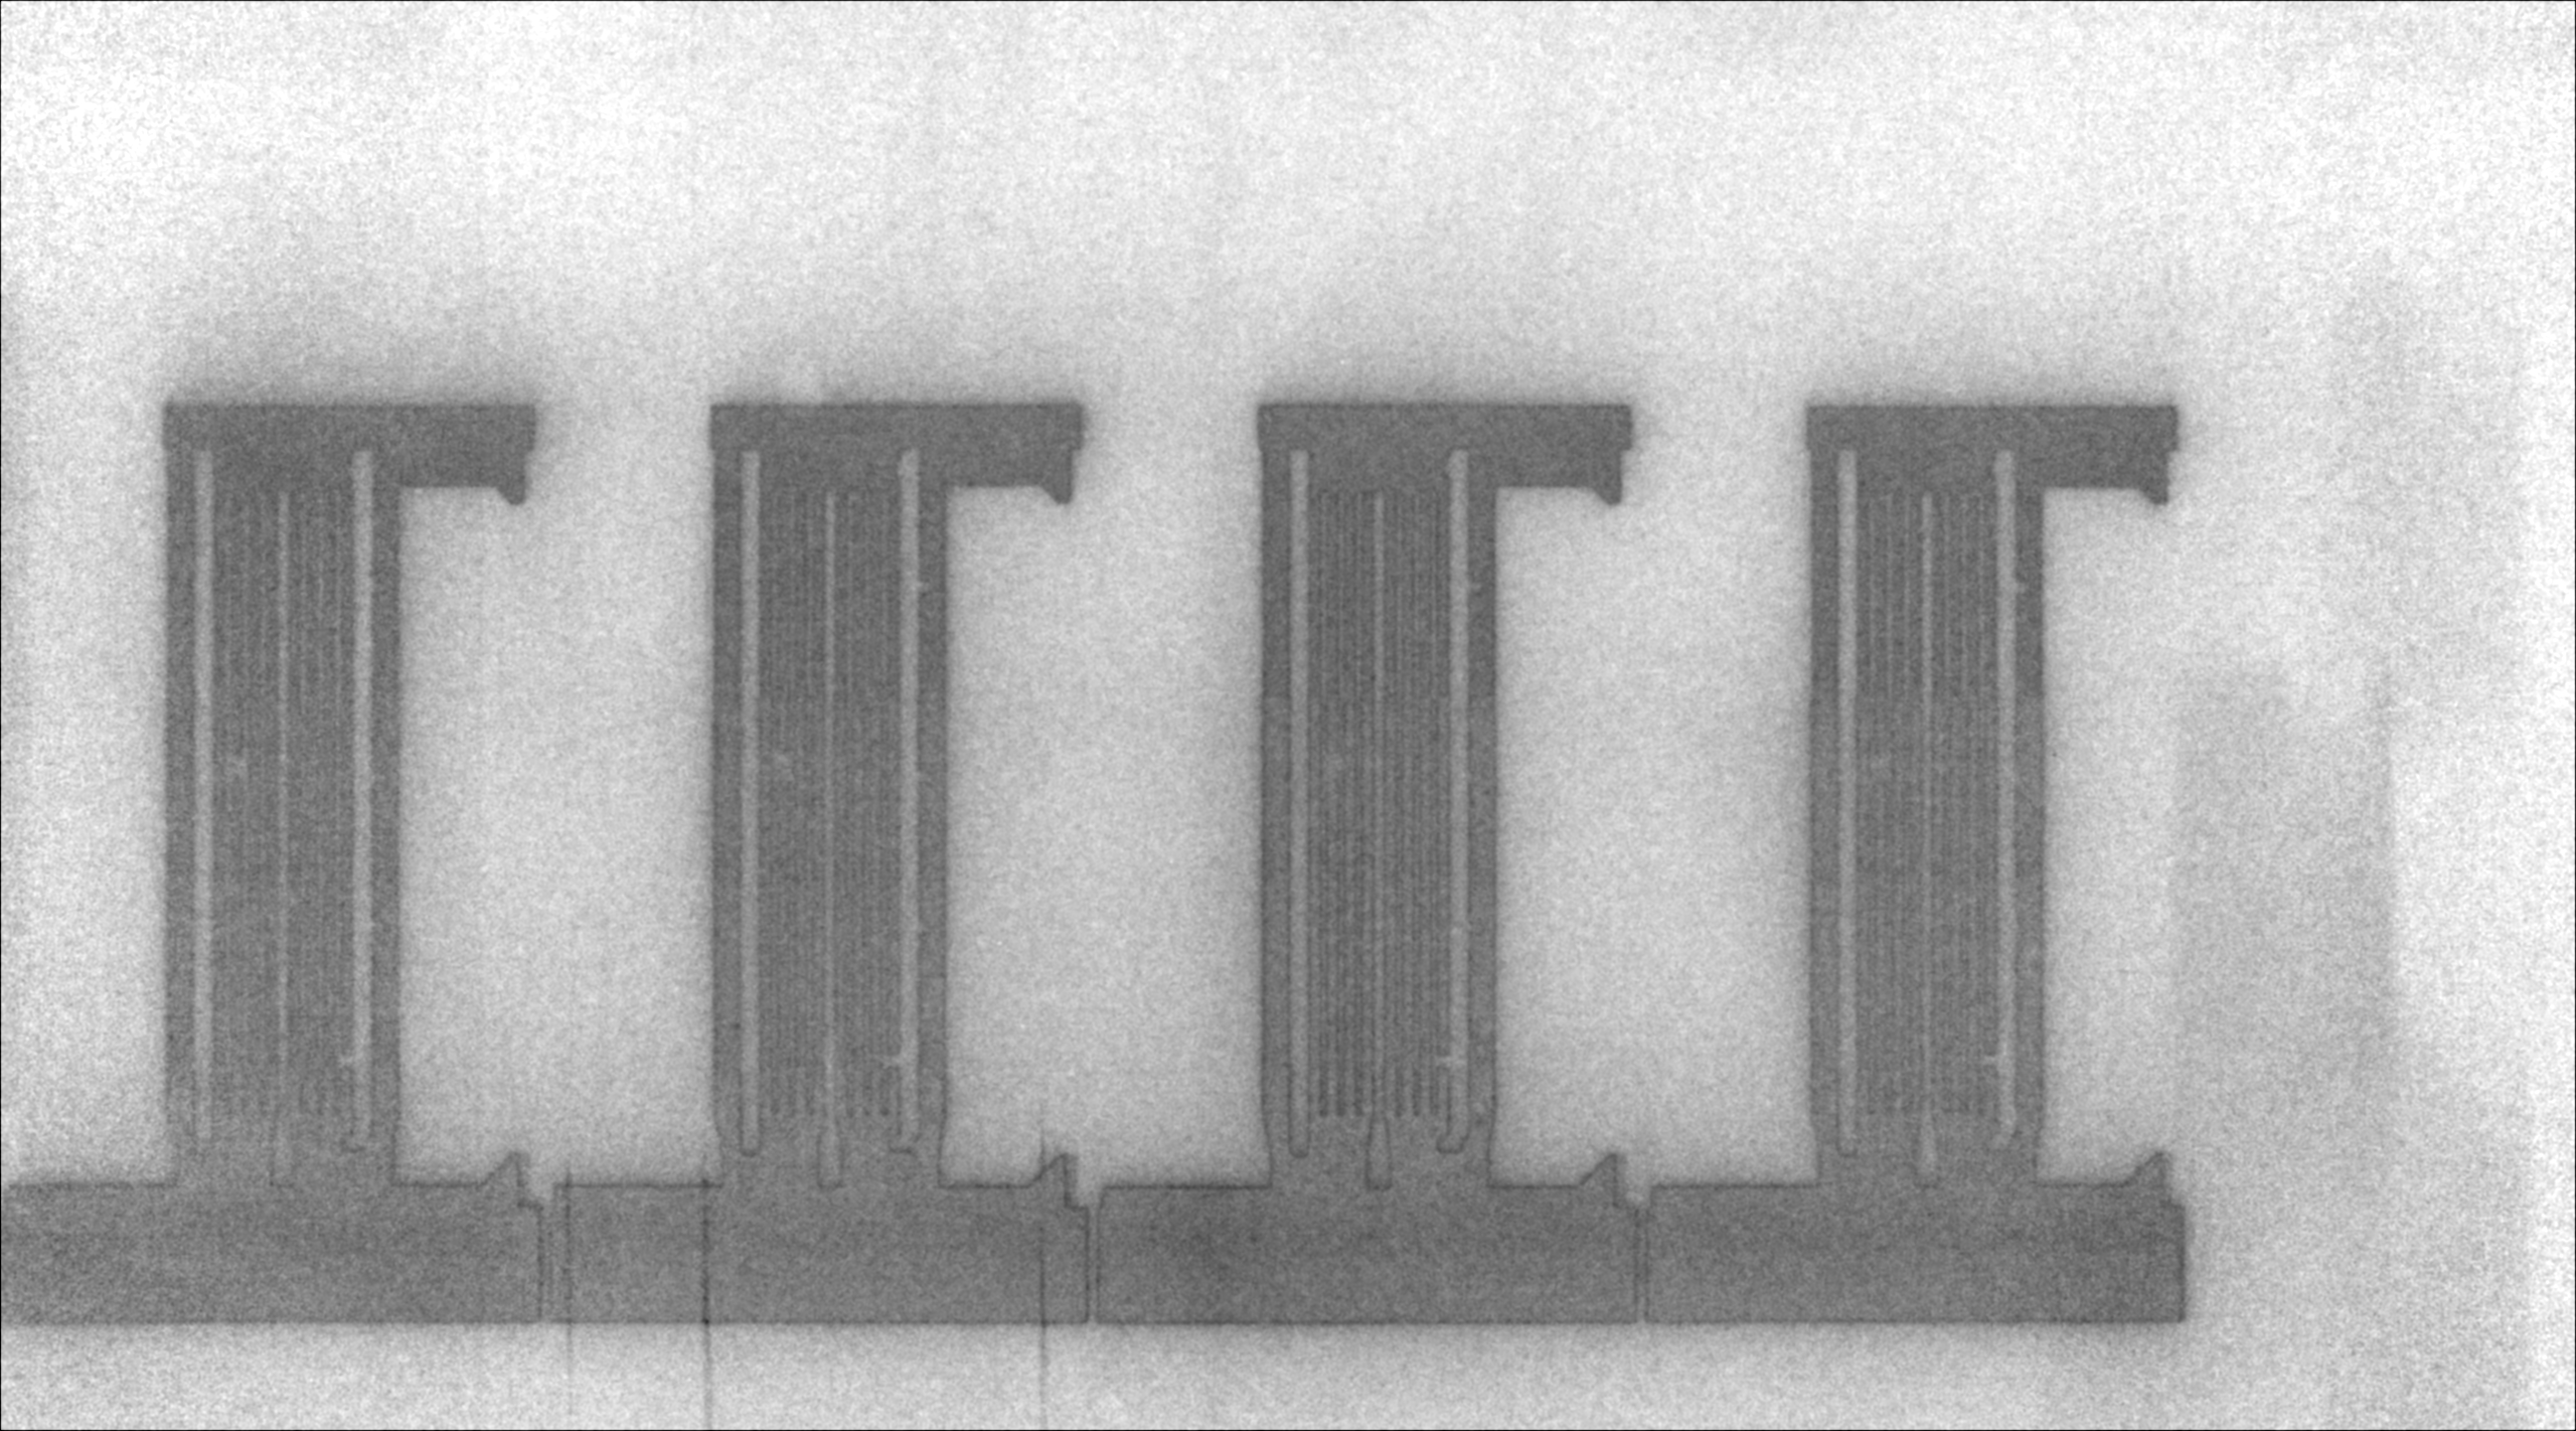
\includegraphics[width=\textwidth]{images/layer_00325}
    \caption{Calibrated capture of a layer.}
    \label{fig:layer}
  \end{subfigure}

  \begin{subfigure}{\textwidth}
    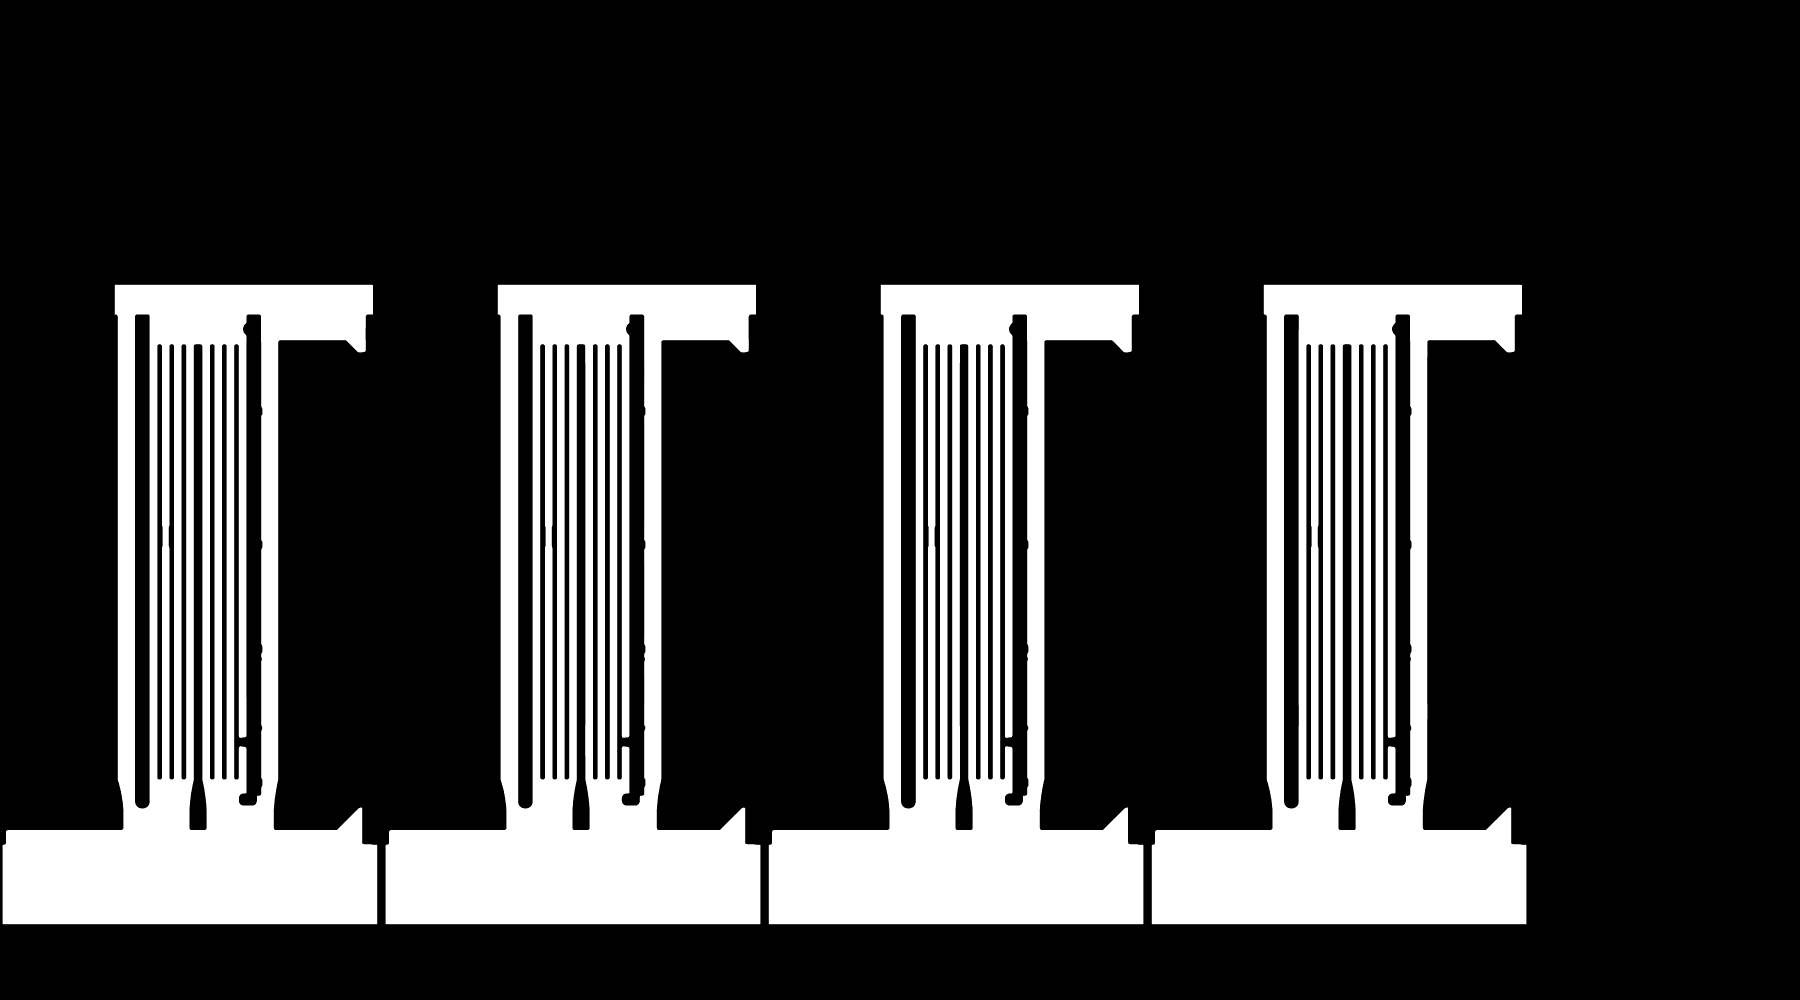
\includegraphics[width=\textwidth]{images/bitmask_00325}
    \caption{Bitmask used by 3D Printer as layer model.}
  \end{subfigure}

  \caption{Printed layer with the respective bitmask.}
  \label{fig:layer_bitmask}

\end{figure}


\begin{figure}[ht]
  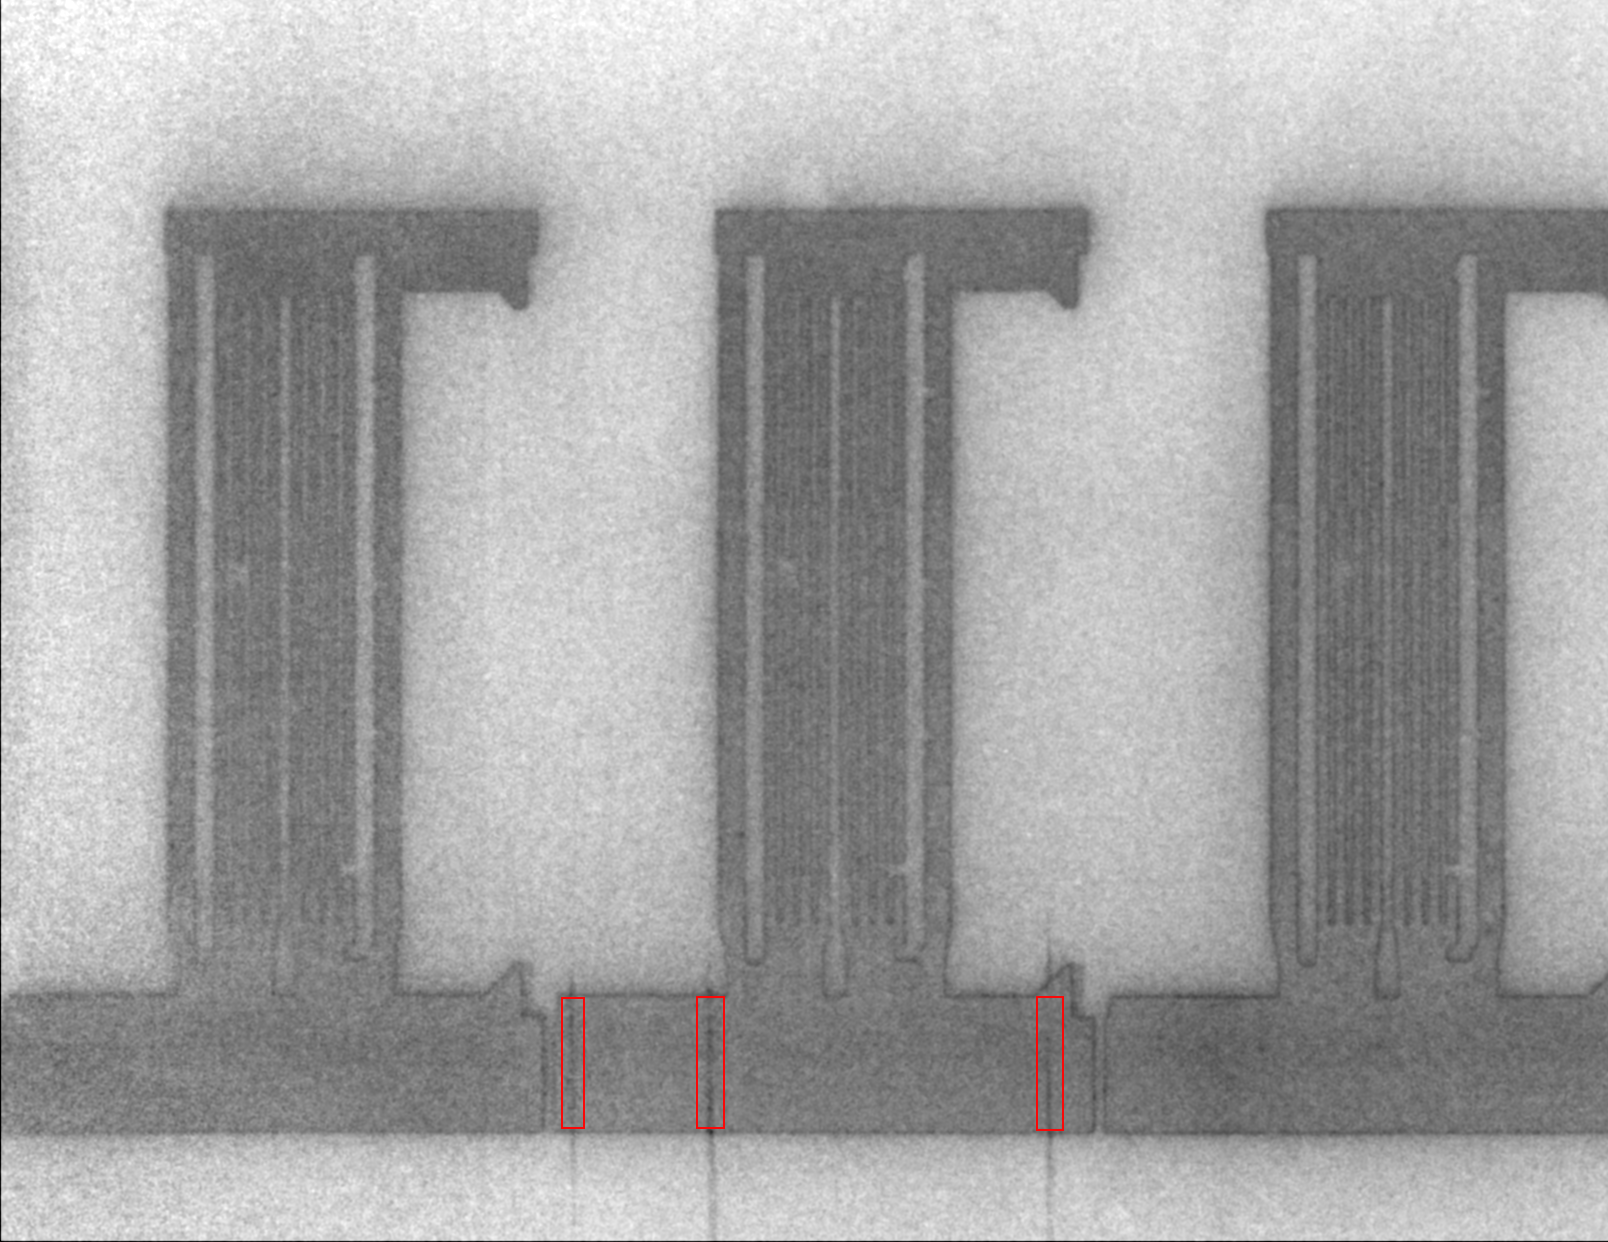
\includegraphics[width=\textwidth]{images/layer_00325_marked_cropped}
  \centering
  \caption{Scratches marked from figure \ref{fig:layer}}
  \label{fig:layer_00325_marked_cropped}
\end{figure}


\subsection{Object Detection with YOLOv5}
TODO: State of the art: RCNN, SSD, YOLO, EfficientDet(compound scaling)? \\
Meanwhile, there are multiple versions of YOLO \cite{yolov4_paper, yolov5_git, yolov7_paper}, but some of them are not canonical versions that are developed by the original authors. One such version is YOLOv5. From a performance point of view, YOLOv5 was performing better than YOLOv4, the latest fully developed canonical version \cite{yolov7_paper}, and it had a better design from a deployment and development point of view: written in PyTorch, supports Tensorboard visualization, better documentation. \\
YOLOv1-5 labels are bounding boxes with class id represented by 1 integer followed by 4 floats. The integer is the class id, the first 2 floats are the coordinates of the center of the bounding box and the next 2 floats are the width and height of the bounding box. The coordinates and sizes of the bounding box are normalized with respect to the image size. Additionally, an extra float can be used to represent confidence for detected bounding boxes.
The

\subsection{Challenges}
A prerequisite for best training results on YOLOv5 detectors is a large enough dataset with consistent labels and image variety \cite{yolov5_dataset}. In the general case, this a trivial part, since there are many open source labeled datasets, like the COCO dataset \cite{coco}. In our case, the printing errors are not common objects that can be found in such datasets, so we need to create our own dataset and there are some challenges regarding this step.\\
\textbf{Dark spots:} Printing a layer is not an instant process and the ??oxidation?? of layers is sometimes uneven, therefore the light is reflected at different strengths along the printed region. As a consequence, the camera might capture some dark marks that are hard to determine if they are scratches as seen in figure \ref{fig:layer_dark_scratch}.\\
\textbf{Capturing elements from previous layers:} \\
\textit{TODO} \\
\textit{- es kann sein, dass dieses Paragraph in ein anderes Section verschiebt wird.} \\
\textbf{Fine scratches:} Not all scratches are equal, making some of them barely visible and from an practical point of view they might be irrelevant. A metric is required for a consistent labeling. \textit{TODO: vielleicht einen Beispiel?}\\
\textbf{Small number of samples:} YOLO based detectors require usually at least 10 000 instances per class, but in our case we have only TODO instances.






\begin{figure}[ht]
  \centering

  \begin{subfigure}{\textwidth}
    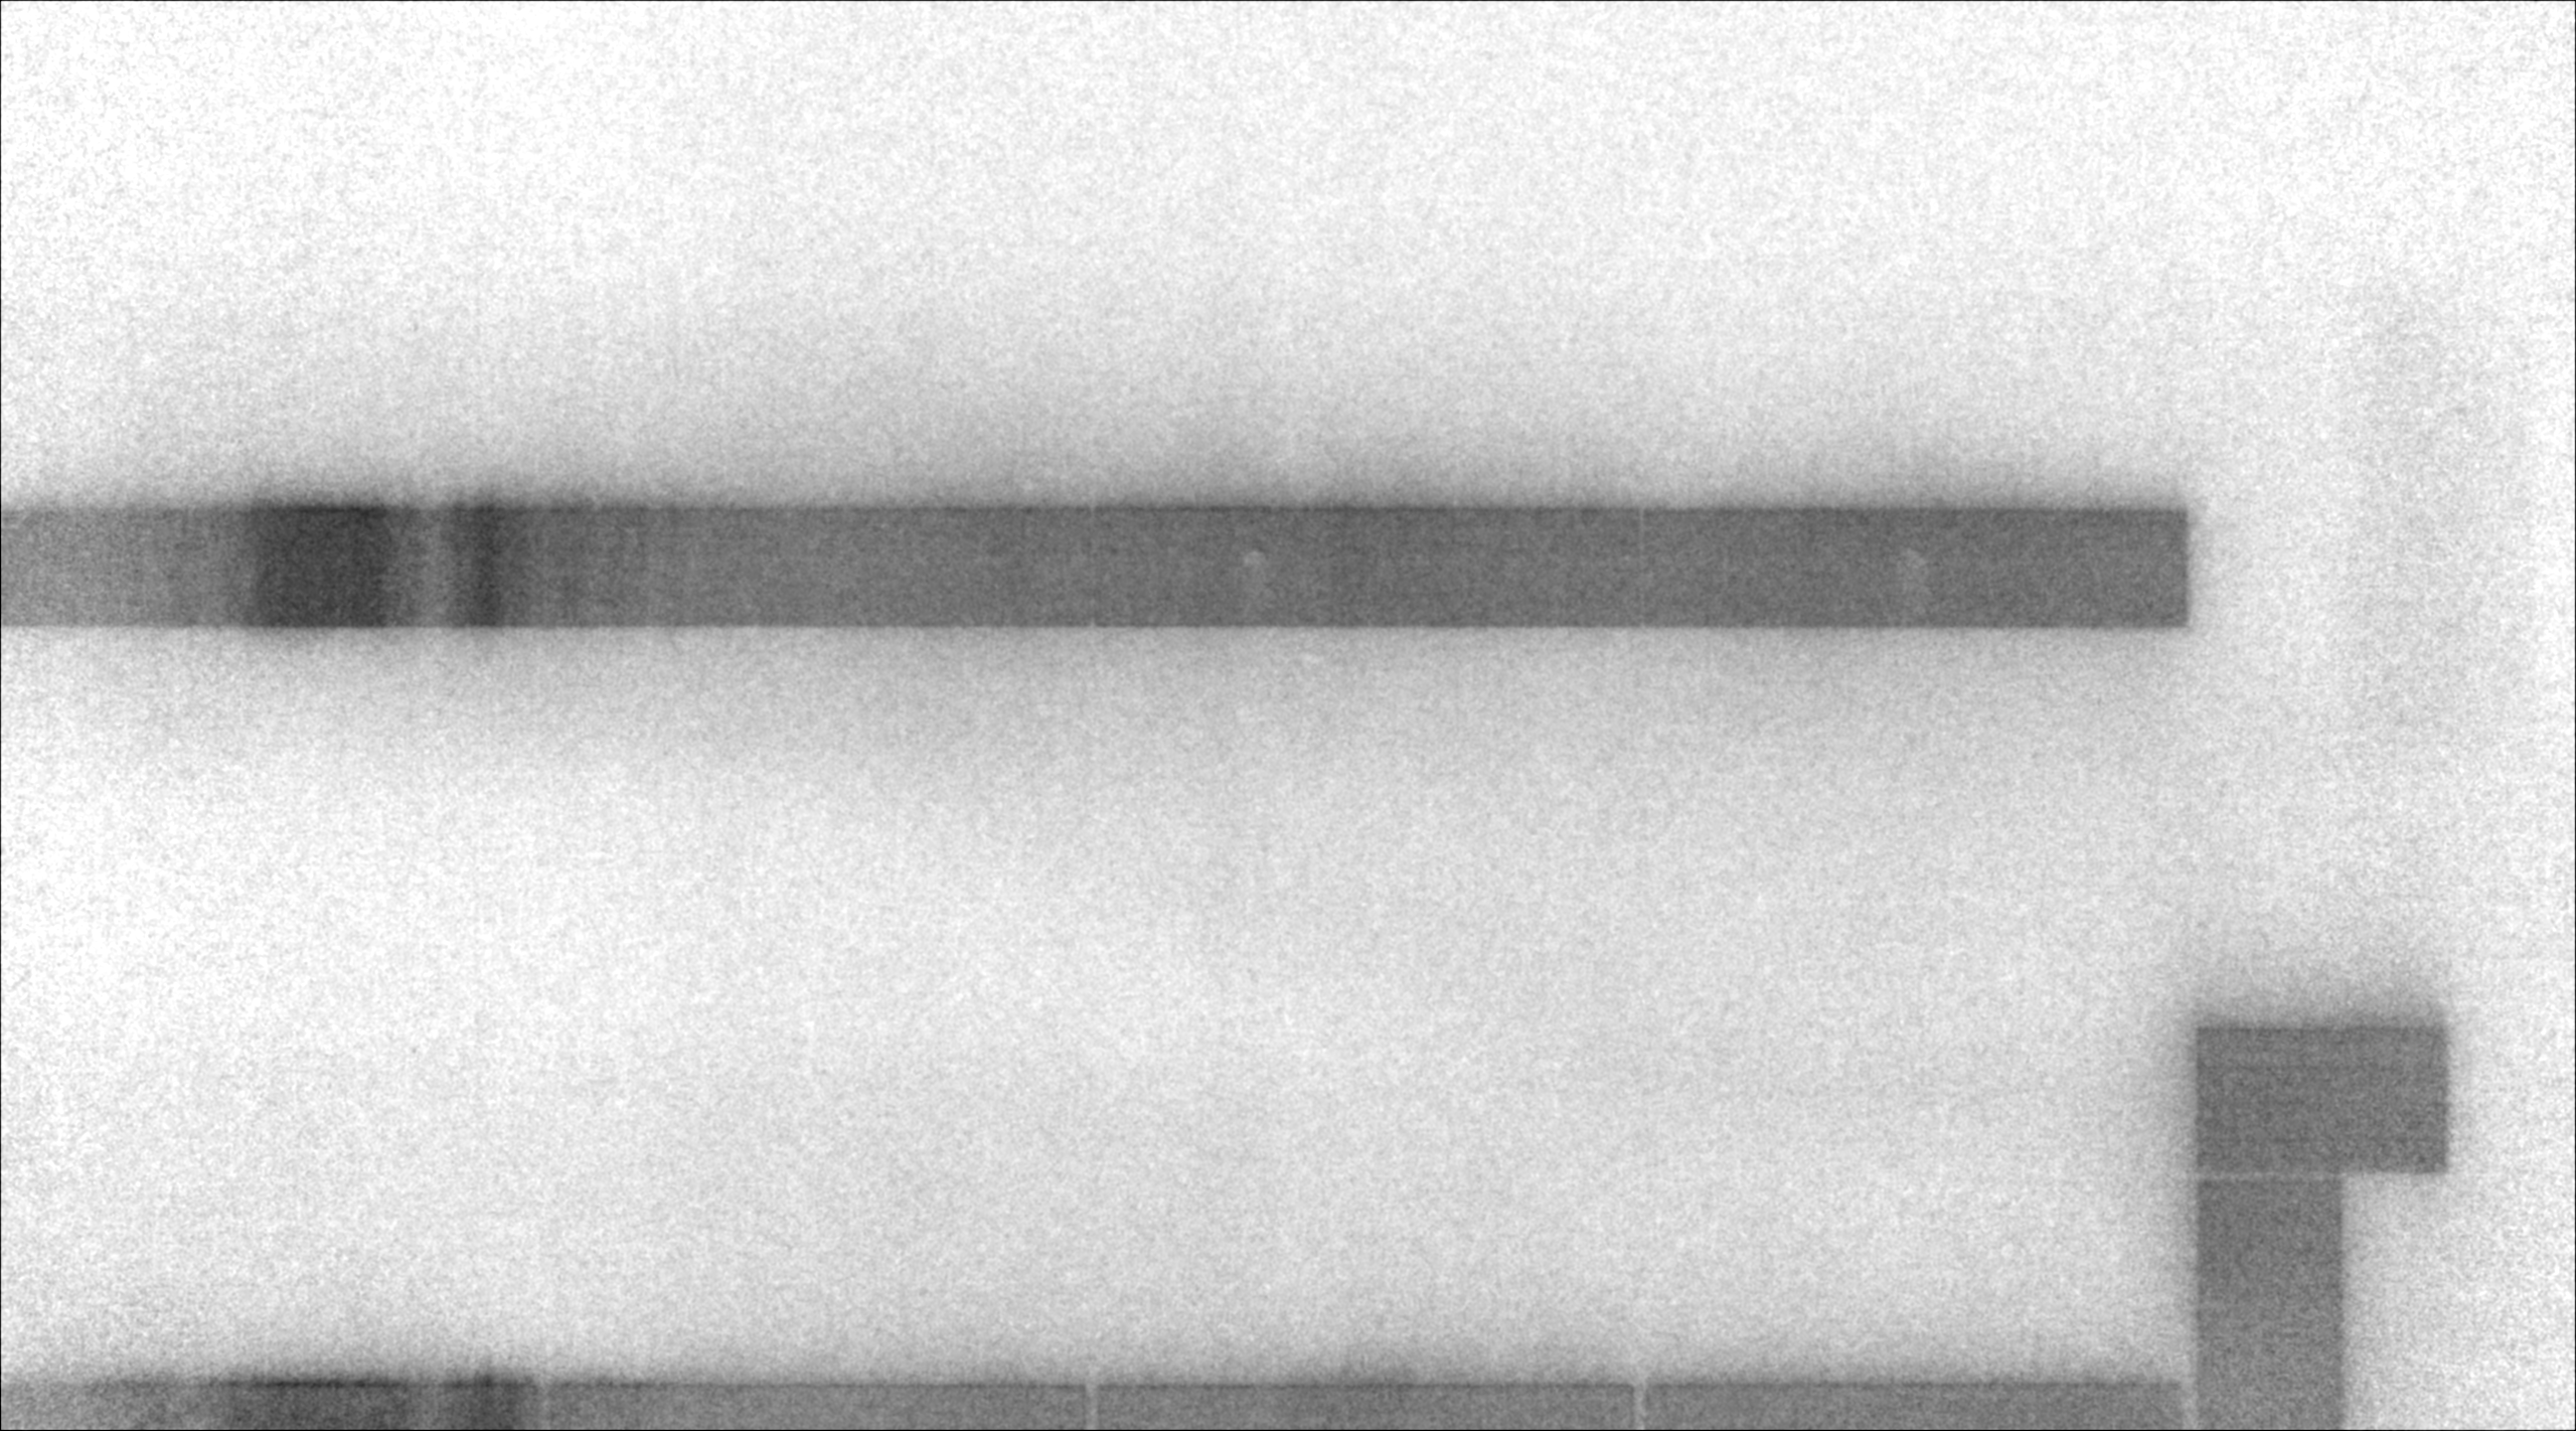
\includegraphics[width=\textwidth]{images/layer_dark_scratch}
    \caption{Layer with dark spots.}

  \end{subfigure}

  \begin{subfigure}{\textwidth}
    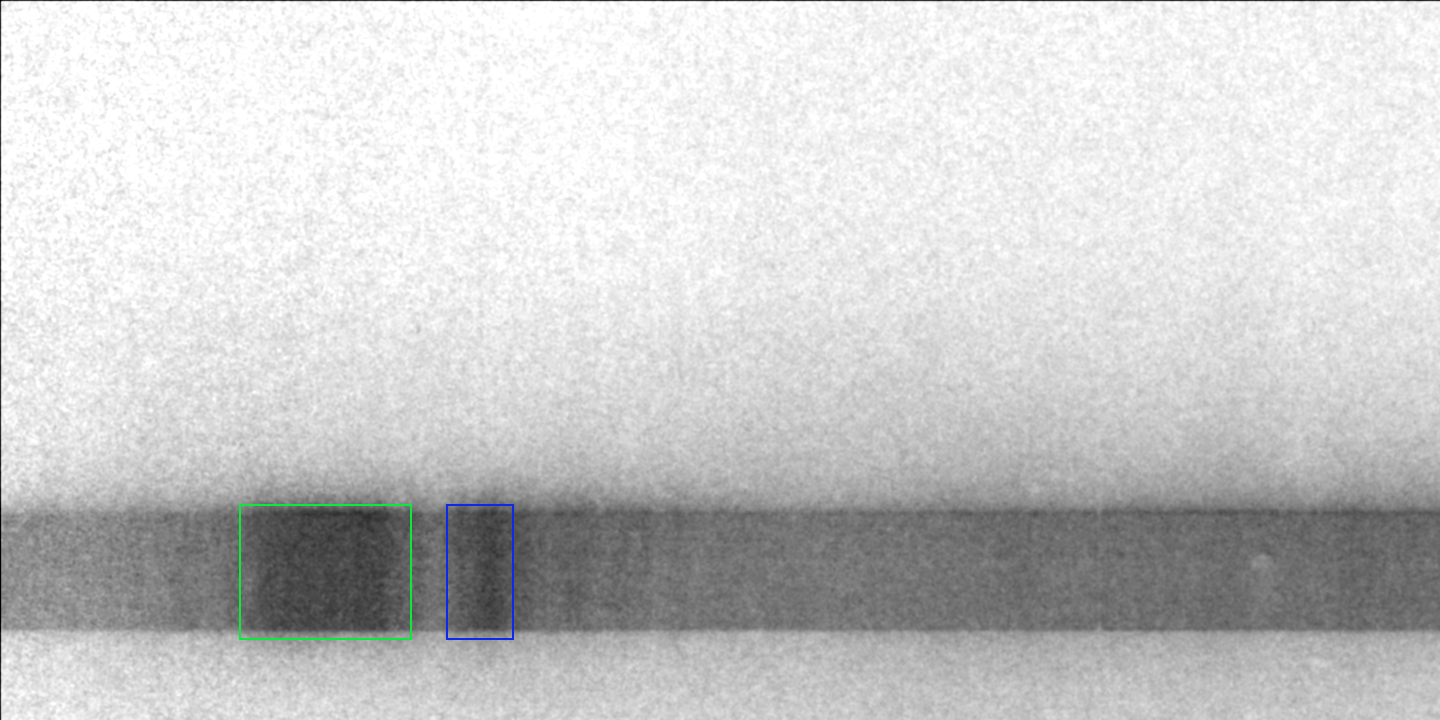
\includegraphics[width=\textwidth]{images/layer_dark_scratch_cropped}
    \caption{Zoomed to the upper left corner of the layer. The green bounding box is safely a dark spot, but the blue bounding box is an ambiguous case.}
  \end{subfigure}

  \caption{Dark spot or scratch?}
  \label{fig:layer_dark_scratch}


\end{figure}

\iffalse
\begin{verbatim}

Links:

URL list from Tuesday, Jul. 19 2022 22:06 PM
To copy this list, type [Ctrl] A, then type [Ctrl] C.

202112_proposal_thesis_AM.pdf
file:///home/captain/Downloads/202112_proposal_thesis_AM.pdf

additive manufacturing - Google Search
https://www.google.com/search?q=additive+manufacturing&oq=additive+manufacturi&aqs=chrome.0.69i59j69i57j0i512l2j0i20i263i512j46i512j69i60l2.3570j0j7&sourceid=chrome&ie=UTF-8

AM Basics - Additive Manufacturing (AM)
https://additivemanufacturing.com/basics/

Additive manufacturing, explained | MIT Sloan
https://mitsloan.mit.edu/ideas-made-to-matter/additive-manufacturing-explained

What is Additive Manufacturing? Definition, Types and Processes - TWI
https://www.twi-global.com/technical-knowledge/faqs/what-is-additive-manufacturing

What is Additive Manufacturing | GE Additive
https://www.ge.com/additive/additive-manufacturing

\end{verbatim}
\fi
